\chapter{Walse}

\vspace{\baselineskip}

\begin{paracol}{2}

\begin{enumerate}
    \item Fly to Walse Castle
\end{enumerate}

\switchcolumn
\begin{misc}{Path to Walse Castle}
    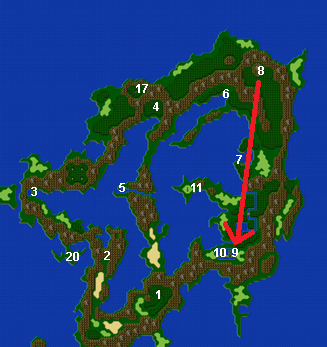
\includegraphics[scale=0.6]{../Graphics/Maps/1. To Walse.png}
    ]
\end{misc}

\switchcolumn*
\newpage
\begin{enumerate}[resume]
    \item You can optionally loot the castle storage room for a \pickup{Tent, 490 Gil, and a Phoenix Down}
\end{enumerate}

\switchcolumn
\begin{misc}{Storage Room Optional Treasure}
    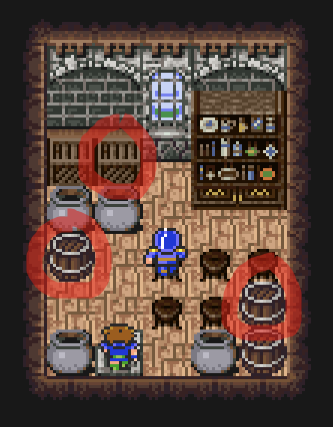
\includegraphics[scale=.399]{../Graphics/Misc/4. Walse Castle Optional Pickups.png}
\end{misc}

\switchcolumn
\resume
\begin{enumerate}[resume]
    \item Enter the throne room
\end{enumerate}

\switchcolumnTwice[*]
\resume
\begin{enumerate}[resume]
    \item Head northwest to Walse Tower
\end{enumerate}

\switchcolumn
\begin{steproute}{Walse and Walse Tower}
    \insertStep{../Graphics/Steps/30. Walse.jpg}
    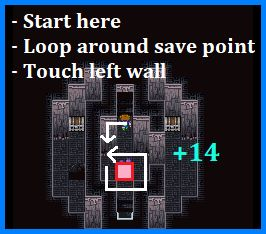
\includegraphics[scale=0.452]{../Graphics/Steps/31. Walse Tower 1.jpg}
\end{steproute}

\switchcolumn
\resume
\begin{enumerate}[resume]
    \item Grab the \pickup{Ether} in the bottom right corner on the last floor
\end{enumerate}

\begin{menu}{After Entering the Wind Crystal Shrine}
	\varwb
    \begin{jobMenu}
        \faris Knight \textbf{(A)}
        \galuf Blue Mage \textbf{(2\pointLeft)} \optimize
        \lenna Blue Mage \textbf{(2\pointLeft)} \optimize
        \bartz Blue Mage \textbf{(2\pointLeft)} \optimize
	\end{jobMenu}
    \begin{itemMenu}
        \potionMenu \ally{Faris (twice)}
    \end{itemMenu}
    \varwe
\end{menu}

\begin{boss}{Garula}
    \varwb
    \begin{round}{1 (Onwards)}
        \faris \leftCommand{\guard}
        \everyoneElse \leftCommand{\blue} \then \goblinPunch
    \end{round}
    \varwe
\end{boss}

\begin{menu}{Before Picking Up the Crystals}
	\varwb
    \begin{jobMenu}
        \bartz Thief \textbf{(2\pointRight)} \ability{!\black} \optimize
	\end{jobMenu}
    \varwe
\end{menu}

\end{paracol}